
\section{Audio Features}
\label{sec:Audio Features}

\subsection{Which audio features appear useful? Select only the most relevant ones or perform a down projection for the next steps.}
\label{sec:Audio Features:a}

As a method to extract the most important audio features, PCA was chosen.\\
The first step was to flatten them into a single array to make them usable for PCA. Using flattened data, the goal was to reach a cumulative explained variance of 95\%.\\
The threshold is reached with 52 Principle Components (Figure \ref{fig:Cumulative Explained Variance}).  The 10 most important feature groups (embeddings, ZCR, mel-spectrogram, mfcc, etc.) of each component are then counted. 

\begin{figure}[htbp]
    \centering
    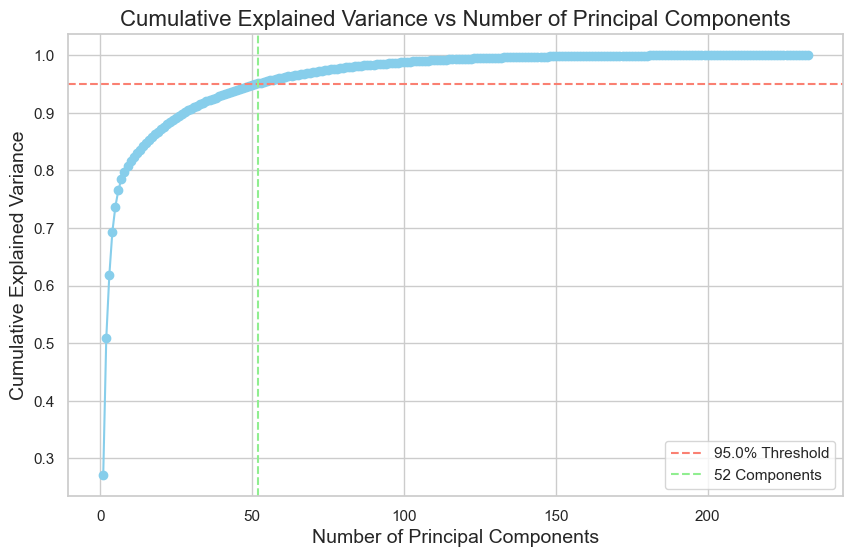
\includegraphics[width=0.5\linewidth, height=5cm]{figs/Cumulative Explained Variance.png}
    \caption{Cumulative Explained Variance using PCA on the audio features}
    \label{fig:Cumulative Explained Variance}
\end{figure}

\textbf{Top contributing feature groups across the first 52 components:}

Feature Group: mfcc, Count: 338;
Feature Group: melspectrogram, Count: 82;
Feature Group: embeddings, Count: 76;
Feature Group: contrast, Count: 14;
Feature Group: centroid, Count: 3;
Feature Group: energy, Count: 2;
Feature Group: power, Count: 1;
Feature Group: flatness, Count: 1;
Feature Group: bandwidth, Count: 1;
Feature Group: zerocrossingrate, Count: 1;
Feature Group: flux, Count: 1

This means that $\Delta$-mfcc and $\Delta\Delta$-mfcc can be ignored.

\subsection{Extract a fixed-length feature vector for each annotated region as well as for all the silent parts in between. }
\label{sec:Audio Features:b}

First, the unimportant features from task a) are excluded. From the important features, the annotated and unannotated parts are extracted.
The snippets of audio features are then concatenated into a single array where the first [:len(X)] elements are annotated and the rest are unannotated features. T-SNE is then used to create a 2-dimensional vector for each section. The vectors are displayed on figure \ref{fig:Audio Features t-SNE} 

%\pagebreak

\subsection{Cluster the audio features for the extracted regions. Can you identify meaningful clusters of audio features? Do the feature vectors of the silent regions predominantly fall into one large cluster?}
\label{sec:Audio Feature Clusters}

K-means was used to cluster the audio features. Clustering was applied to the raw data instead of the t-SNE down projection, as it provided a better distinction between annotated and unannotated features.\\
While cluster 9 consists almost entirely of unannotated features, this is not so clear for all the other clusters (Figure \ref{fig:Audio Feature Clusters}). This is probably due to the annotation errors, as most of the unannotated parts are either not completely silent or are small gaps between annotations that should still be part of the annotation. 

\begin{figure}[h]
  \centering
  \begin{minipage}[b]{0.49\textwidth}
    \centering
    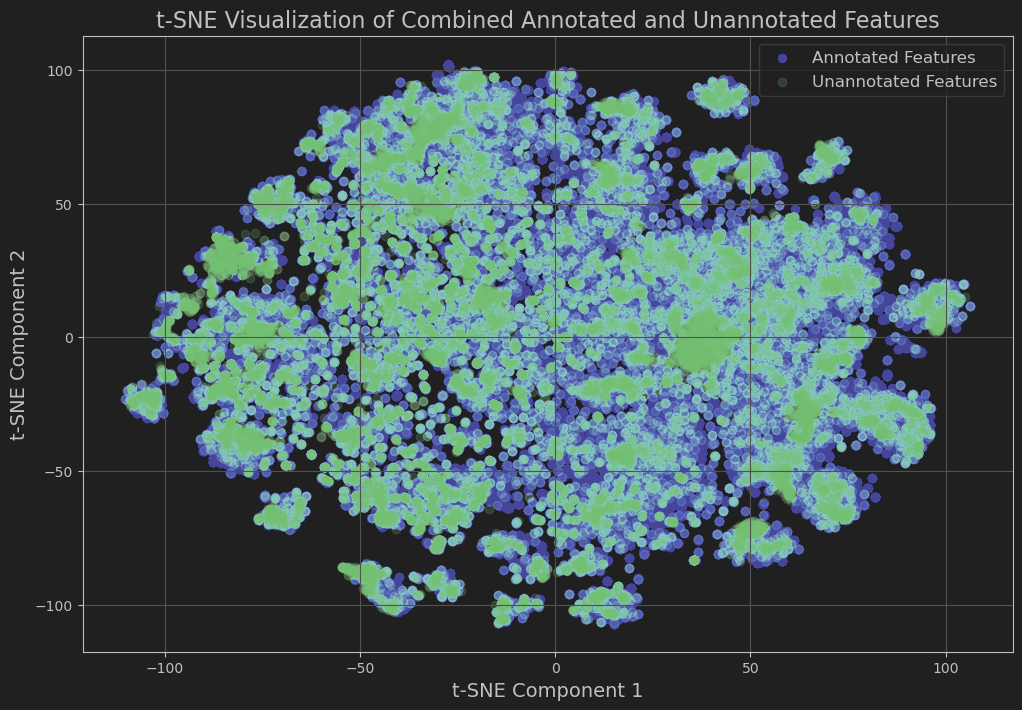
\includegraphics[width=\textwidth]{figs/Audio Features T-SNE.png}
    \caption{Feature Vectors using t-SNE}
    \label{fig:Audio Features t-SNE}
  \end{minipage}
  \hfill
  \begin{minipage}[b]{0.49\textwidth}
    \centering
    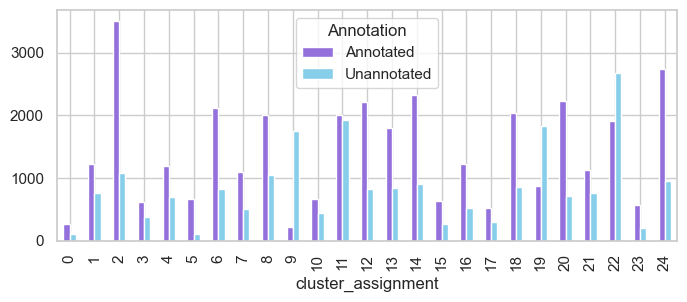
\includegraphics[width=\textwidth]{figs/Clustered Audio Features.png}
    \caption{Clusters of Audio Features}
    \label{fig:Audio Feature Clusters}
  \end{minipage}
\end{figure}

